\section{Zielsetzung}
In diesem Versuch werden gekoppelte elektrische Schwingkreise betrachtet. 
Ziel ist es, das Verhalten der Energie bzw. des Energieübergangs zwischen den einzelnen Systemen, insbesondere unter dem Aspekt der Zeitabhängigkeit zu betrachten. 
Des Weiteren soll das Verhalten des Gesamtsystems bei erzwungenen Schwingungen, also äußerer periodischer Anregung, untersucht werden.
\section{Theorie}
\label{sec:Theorie}
Sind zwei schwingfähige Systeme miteinander gekoppelt, so beeinflussen sie sich gegenseitig.
Wird eines der Systeme zum Schwingen angeregt, so pendelt die zugeführte Energie zwischen beiden Systemen. Die Energie ist erhalten.
\subsection{Kapazitiv gekoppelte Schwingkreise}
\label{sec:Theorie1}
\begin{figure}[h]
	\centering
	\label{fig:gekoppelte SK}
		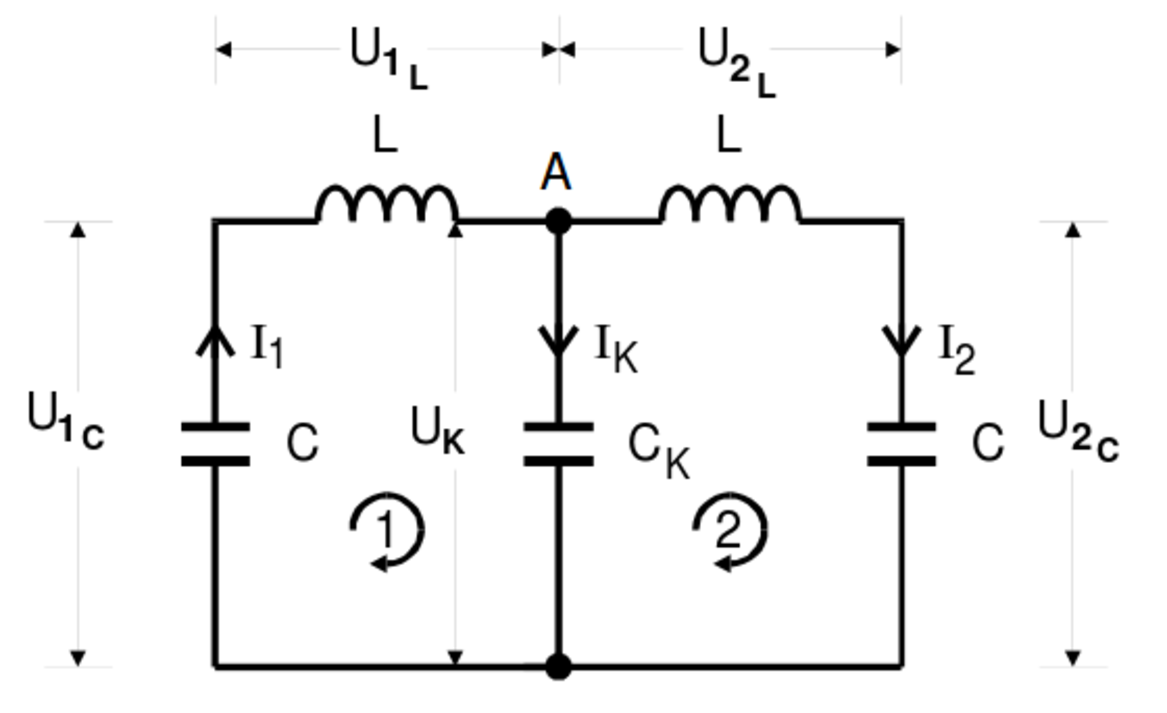
\includegraphics[width=0.8\textwidth]{Bilder/2SK.pdf}
		\caption{Zwei LC-Schwingkreise kapazitiv gekoppelt. \cite{v355}}
\label{fig:gekoppelte SK}
\end{figure}
Die zwei dargestellten, eigenständigen Schwingkreise sind über den Kondensator der Kapazität $C_\mathup{K}$ miteinander verknüpft.
Mit Knoten- und Maschenregel nach \textsc{Kirchhoff} lassen sich folgende Gleichungen herleiten:
\begin{equation}
	I_\mathup{K}=I_1-I_2
	\label{eq:I_k}
\end{equation}
\begin{equation}
	U_{1\mathup{C}}+U_{1\mathup{L}}+U_{\mathup{K}}=0
	\label{eq:U_1}
\end{equation}
\begin{equation}
	U_{2\mathup{C}}+U_{2\mathup{L}}+U_{\mathup{K}}=0
	\label{eq:U_2}
\end{equation}
Des Weiteren gelten die Beziehungen
\begin{equation}
	U_\mathup{C}=\frac{1}{C}\int{I\mathup{d}t}
	\label{eq:U_C}
\end{equation}
und
\begin{equation}
	U_\mathup{L}=L\dot{I}.
	\label{eq:U_L}
\end{equation}
Einsetzen von \eqref{eq:U_C} und \eqref{eq:U_L} sowie Ableiten nach der Zeit ergibt ein Differentialgleichungssystem. 
Werden die Gleichungen entkoppelt, lassen sie sich unabhängig voneinander lösen.
Lösung der ersten Gleichung, entstanden durch Addition der Ströme $I_\text{i}$,
\begin{equation}
	L(\ddot{I_1}+\ddot{I_2})+\frac{1}{C}({I_1}+{I_2})=0
	\label{eq:I_1+I_2}
\end{equation}
ist eine harmonische Schwingung der Form
\begin{equation}
	({I_1}+{I_2})(t)=({I_{1,0}}+{I_{2,0}})\cos(\frac{t}{\sqrt{LC}})
\label{eq:lsg_I_1+I_2}
\end{equation}
mit der Schwingungsfrequenz, gemäß $\omega=2\pi f$,
\begin{equation}
f_+=\frac{1}{2\pi\sqrt{LC}}.
\label{eq:f_+}
\end{equation}
Diese Frequenz entspricht derer eines einzelnen, ungedämpften Oszillators mit den Bauteilen $L$ und $C$.
 Die Amplitude $(I_{1,0}+I_{2,0})$ bleibt konstant.
Die zweite Gleichung, entstanden analog durch Subtraktion,
\begin{equation}
	L(\ddot{I_1}-\ddot{I_2})+\bigl(\frac{1}{C}+\frac{1}{C_\mathup{K}}\bigr)({I_1}-{I_2})=0
	\label{eq:I_1-I_2}
\end{equation}
wird gelöst durch
\begin{equation}
	({I_1}-{I_2})(t)=({I_{1,0}}-{I_{2,0}})\cos\biggl(t{\biggl[L\biggl({\frac{1}{C}+\frac{1}{C_\mathup{K}}}\biggr)⁻¹\biggr]^{-\frac{1}{2}}}\biggr).
\label{eq:lsg_I_1-I_2}
\end{equation}
Die Schwingungsfrequenz 
\begin{equation}
f_-=\frac{1}{2\pi\sqrt{L\bigl({\frac{1}{C}+\frac{1}{C_\mathup{K}}}\bigr)⁻¹}}
\label{eq:f_-}
\end{equation}
 ist größer als Schwingungsfrequenz $f_+$.
Erneute Addition und Subtraktion der voneinander unabhängigen Gleichungen ergibt
\begin{equation}
	I_1(t)=\frac{1}{2}({I_{1,0}}+{I_{2,0}})\cos(2\pi f_+t)+\frac{1}{2}({I_{1,0}}-{I_{2,0}})\cos(2\pi f_-t)
	\label{eq:I_1_ur}
\end{equation}
und
\begin{equation}
	I_2(t)=\frac{1}{2}({I_{1,0}}+{I_{2,0}})\cos(2\pi f_+ t)-\frac{1}{2}({I_{1,0}}-{I_{2,0}})\cos(2\pi f_- t).
	\label{eq:I_2_ur}
\end{equation}
Im Folgenden werden zwei Spezialfälle betrachtet. 
Schwingen die Systeme mit gleicher Amplitude $I_{1,0}=I_{2,0}$ und gleicher Phase, so verschwindet die Differenzschwingung \eqref{eq:lsg_I_1-I_2}, sodass die Oszillatoren jeweils mit $f_+$ eines einzelnen Oszillators und in Phase schwingen.
 Am Kondensator $C_\mathup{K}$ liegt zu keinem Zeitpunkt eine Spannung an, da die Ströme sich gegenseitig kompensieren.
Schwingen die Systeme mit entgegengesetzter Amplitude  $I_{1,0}=-I_{2,0}$ und Phase, so verschwindet die Summenschwingung \eqref{eq:lsg_I_1+I_2}. Die Oszillatoren schwingen gegenphasig mit der Frequenz $f_-$.
Diese beiden Schwingungsmoden werden als Fundamentalschwingungen des Systems bezeichnet.

\begin{figure}[h]
	\centering
	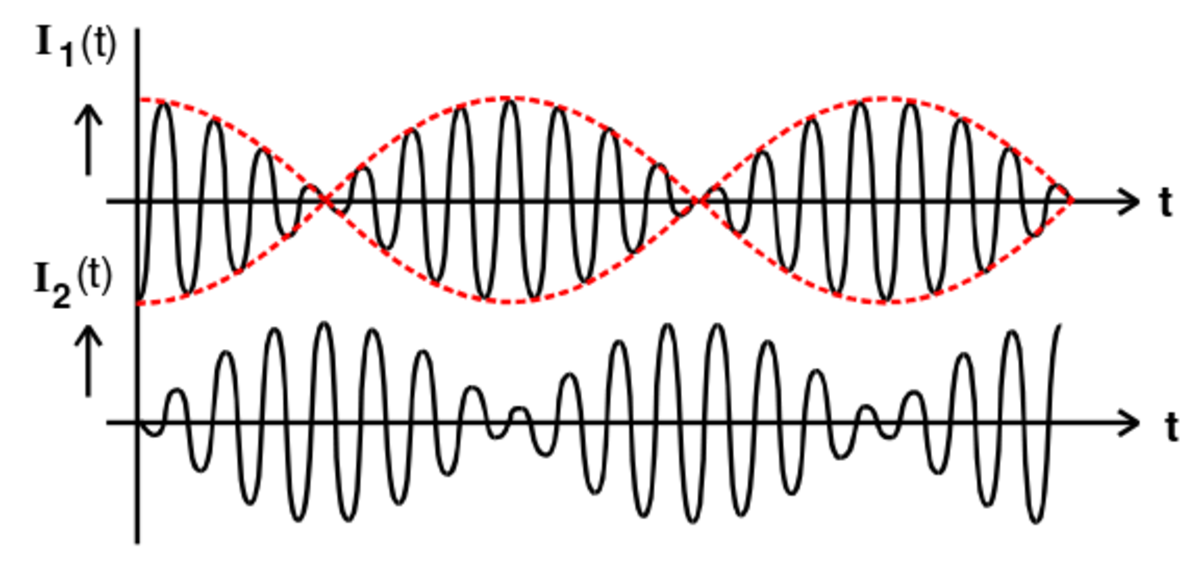
\includegraphics[width=0.8\textwidth]{Bilder/Schwebung.pdf}
		\caption{Schwebung. \cite{v355}}
		\label{fig:schwebung}
\end{figure}

Wird zur Zeit $t=0$ nur ein Oszillator ausgelenkt, d.h. $I_{1,0}\neq0$,\,$I_{2,0}=0$, vereinfachen sich \eqref{eq:I_1_ur} und \eqref{eq:I_2_ur}. 
Durch Ausnutzen von Additionstheoremen ergeben sich
\begin{equation}
	I_1(t)=I_{10}\cos(\frac{1}{2}(\omega⁺+\omega⁻)t)\cos(\frac{1}{2}(\omega⁺-\omega⁻)t)
\end{equation}
und
\begin{equation}
	I_2(t)=I_{10}\sin(\frac{1}{2}(\omega⁺+\omega⁻)t)\sin(\frac{1}{2}(\omega⁺-\omega⁻)t).
\end{equation}
Gemäß der Annahme $f_+\approx f_-$ und $C_\mathup{K}\gg C$ ist $\frac{1}{2}(\omega⁺-\omega⁻)\approx\omega⁺$ und $\omega⁻-\omega⁺\ll\omega⁺$.
Die Oszillatoren schwingen mit der Frequenz $\frac{1}{2}(f_+ + f_-)$, welche ungefähr der Frequenz eines Einzeloszillators entspricht. 
Die Amplituden verändern sich periodisch mit der Schwebungsfrequenz $f_- - f_+$. 
Die Verhältnisse haben sich nach der Zeit 
\begin{equation}
\frac{T}{2}({\omega⁻-\omega⁺})=\frac{\pi}{2}
\end{equation}
 umgekehrt, die Energie pendelt periodisch mit der Schwebungsfrequenz zwischen beiden Systemen.

\newpage
\subsection{Erzwungene Schwingungen}
\label{sec:erzwungen}
Erzwungene Schwingungen werden durch eine von außen angelegte Sinusspannung $U(t)$ erzeugt.
%Wird Abbildung \ref{fig:gekoppelte SK} um einen Sinusgenerator erweitert, so kann mit Hilfe der Maschenregel eine Formel für den Strom $I_2$  gewonnen werden.
%\begin{equation}
%I_2=|U|\frac{1}{\sqrt{4{\omega}²{C_\mathup{K}}² R² Z(\omega)²+\biggl(\frac{1}{\omega C_\mathup{K}}-\omega C_\mathup{K} Z(\omega)² + \omega R² C_\mathup{K}\biggr)²}}=|U||L|,
%\end{equation}
%mit dem Leitwert $|L|$ und dem Widerstand $Z(\omega)$, nähert sich für sehr große und sehr geringe Frequenzen dem Wert Null an.
%An den Stellen der genannten Fundamentalfrequenzen $\omega⁺$ und $\omega⁻$ treten Resonanzphänomene auf.
%Die Resonanzkurve zweier gekoppelter Schwingkreise unterscheidet sich von der Kurve eines einzelnen Oszillators mit periodischer Anregung durch die Anzahl der auftretenden Maxima.
%Die Werte des Stromes an diesen Frequenzen entscheiden sich nur unwesentlich, sodass die Leitwerte $|L(\omega⁺)|=|L(\omega⁻)|\approx\sfrac{1}{2R}$  angenommen werden darf. 
%Betrachtet man die Frequenz $\omega⁺$, welche unabhängig von der Koppelkapazität $C_\mathup{K}$ ist, können beide Schwingkreise als ein Kreis mit $L_\mathup{Ges}=2L$ und $C_\mathup{Ges}=\sfrac{1}{2}C$ angesehen werden. 
%Durch die Koppelleitung fließt kein Strom. 
%Bei der Frequenz $\omega⁻$ ist $C_\mathup{Ges}=\sfrac{C C_\mathup{K}}{C_\mathup{K}+2C}$ - durch die Koppelleitung fließt nun der maximale Strom.
Im Resonanzfall unterscheidet sich die $I–\phi$-Resonanzkurve zweier gekoppelter Schwingkreise von der eines einzelnen Oszillators durch die Anzahl der auftretenden Maxima. An den Stellen der in Kapitel \ref{sec:Theorie1} hergeleiteten Fundamentalfrequenzen $f_+$ und $f_-$ befinden sich zwei Maxima.
